\chapter{BGP RFD}
\label{cha:bgp_rfd}

\ac{RFD} is another mechanisms of \ac{BGP} used to prevent messages storms
and to reduce the impact of the external noise.
It is used to avoid flapping routes to continuously make the network unstable.
When a network flaps is detected a certain value is increased and when it overpass a threshold
then the route is suppressed and not advertised anymore until it goes back
below the threshold (or after a certain time).

\ac{RFD}, other than \ac{MRAI}, is one of the most studied parameters of \ac{BGP}
because of its influence in the convergence time \cite{mao2002route,pelsser2011route}.
\ac{RFD} has received different updates from its first implementation, but recent
studies showed that most of the providers still use outdated parameters \cite{gray2020bgp}.

Deprecated values if used can lead to a heavy restrictive suppression
of some routes, delaying the correct spreading of information.
Some cases of suppression are caused by faulty interfaces that heavily flaps hundreds of times,
while other times is just an update of the node configuration that
cause the route to flaps a couple of times.

In the following sections, I am about to show how legacy \ac{RFD} can affect
small flaps and how would the new version of \ac{RFD} react to them.
By consequence, how the figure of merit threshold can impact the network
performances.
In this chapter, giving that the goal is to present \ac{RFD} and its effects
\ac{MRAI} is setted to the standard value of \SI{30}{\second} as described
in~\cite{rfc4271}.

\section{RFD on toy topologies}
\label{sec:rfd_toy_topologies}

%\begin{itemize}
%		\item clique with MRAI=30
%		\item clique RFD vs no RFD
%		\item node x and 5 figure of merit
%\end{itemize}

I firstly studied \ac{RFD} on toy topologies, to see the effects of it in small
networks, like I did in \Cref{sec:bgp_mrai_clique}.
As a graph, I used a clique of dimension \num{10}, the source of the signalling
is connected to the node \num{0} while the node \num{5} act as unique servicer
for the node $x$.
The node \num{5} won't be able to share information to node $x$ because of \ac{RFD}.
Node $x$ would have to wait until the \ac{RFD} value of \num{5} fell below
the reuse threshold in order to be able to make the \ac{RIB} converge.

The parameters used for \ac{RFD} are the default \textit{CISCO} parameters,
showed in table \Cref{tbl:cisco_rfd} and are going to be used by
all the nodes.

\begin{table}[h]
	\begin{center}
	\begin{tabular}{ || m{5cm}| m{2cm} || } 
	\hline
	Parameter & Value \\ 
	\hline \hline
	withdrawal penalty & 1.0 \\
	\hline
    re-advertisement penalty & 0.0 \\
	\hline
    attribute change penalty & 1.0 \\
	\hline
    suppress threshold & 2.0 \\
	\hline
    half-life (min) & 15 (900s) \\
	\hline
    Reuse Threshold & 0.75 \\
	\hline
    Max Suppress Time (min.) & 60 (3600s) \\
	\hline
	\end{tabular}
\end{center}

	\caption{Cisco default \ac{RFD} parameters}
	\label{tbl:cisco_rfd}
\end{table}

The parameters of the environment are presented in \Cref{tbl:clique_rfd_params}.

\begin{table}[h]
	\begin{center}
	\begin{tabular}{ || m{4cm}| m{8cm} || } 
	\hline
	Property & Value \\ 
	\hline \hline
	Seeds & $[1, 10]$ \\ 
	\hline
	Signaling & \q{AWAWAWA} \\
	\hline
		Withdraws delay & Constant distribution of \SI{300}{\second} \\ 
	\hline
	Announcement delay & constant distribution of \SI{300}{\second} \\ 
	\hline
		MRAI & $[0, 120]$ \\
	\hline
	Link delay & Uniform distribution between \SI{0.012}{\second} and \SI{3}{\second} \\
	\hline
	\end{tabular}
\end{center}

	\caption{Environment parameters used for the experiments on \ac{RFD}
		with the clique graph}
	\label{tbl:clique_rfd_params}
\end{table}

Messages in the signal are delayed by \SI{300}{\second} for two reasons:
\begin{itemize}
    \item I don't want that \ac{MRAI} compress parts of the signal;
	\item I'm trying to simulate one of the possible behaviours that triggers a
		\ac{RFD} suppression, the human faulty reconfiguration of the node.
\end{itemize}
The signal contains \num{3} flaps, the first one is hypothetically attributed
to a configuration that doesn't work properly, the second one is caused by a
buggy correction of the configuration and the last one by the introduction of a
correct configuration.

\fxfatal{execute experiments for RFD and no RFD with MRAI=30sec, at least 50}

The network performances with the environment in \Cref{tbl:clique_rfd_params} are
presented in \Cref{fig:RFD_2439_MRAI30}.
Is important to underline that a node is considered converged when all the routes
are available again and its \ac{RIB} doesn't change anymore.
The network convergence time is given by the average of all the nodes convergence
time.
\begin{figure}[h]
     \centering
     \begin{subfigure}[b]{0.49\textwidth}
         \centering
         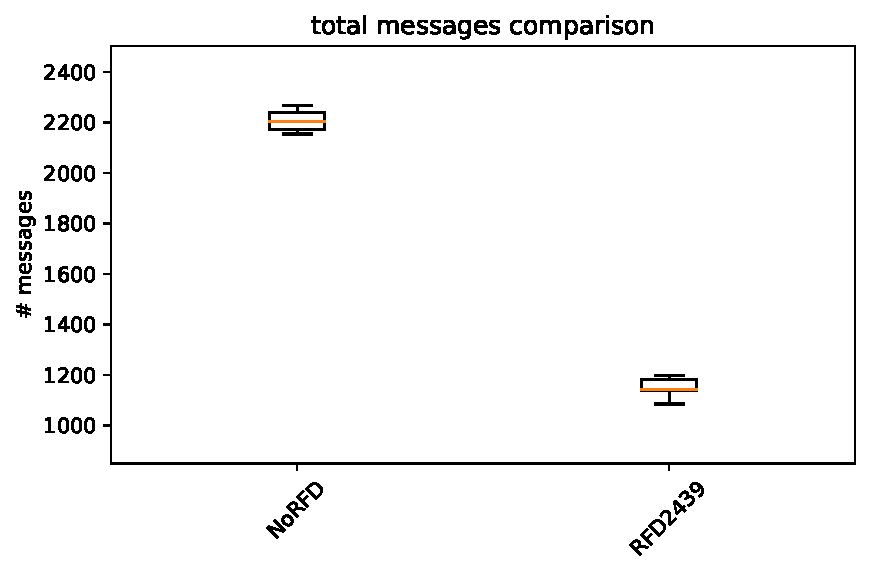
\includegraphics[width=\textwidth]{images/RFD/clique/clique_rfd_comparison_2439_messages_boxplot.pdf}
         \caption{Messages comparison}
         \label{fig:RFD_2439_clique_MRAI30_messages}
     \end{subfigure}
     \hfill
     \begin{subfigure}[b]{0.49\textwidth}
         \centering
         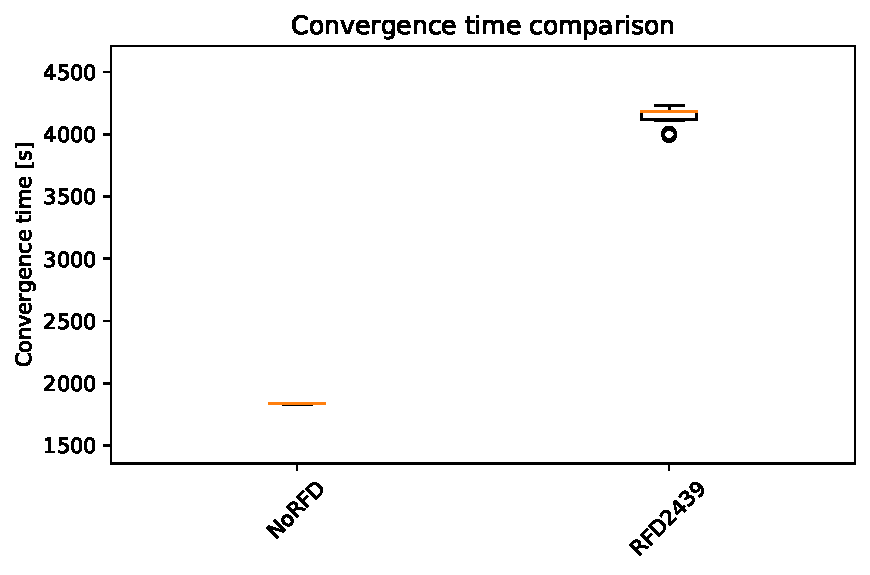
\includegraphics[width=\textwidth]{images/RFD/clique/clique_rfd_comparison_2439_time_boxplot.pdf}
         \caption{Convergence time}
         \label{fig:RFD_2439_clique_MRAI30_convTime}
     \end{subfigure}
     \hfill
     \begin{subfigure}[b]{0.49\textwidth}
         \centering
         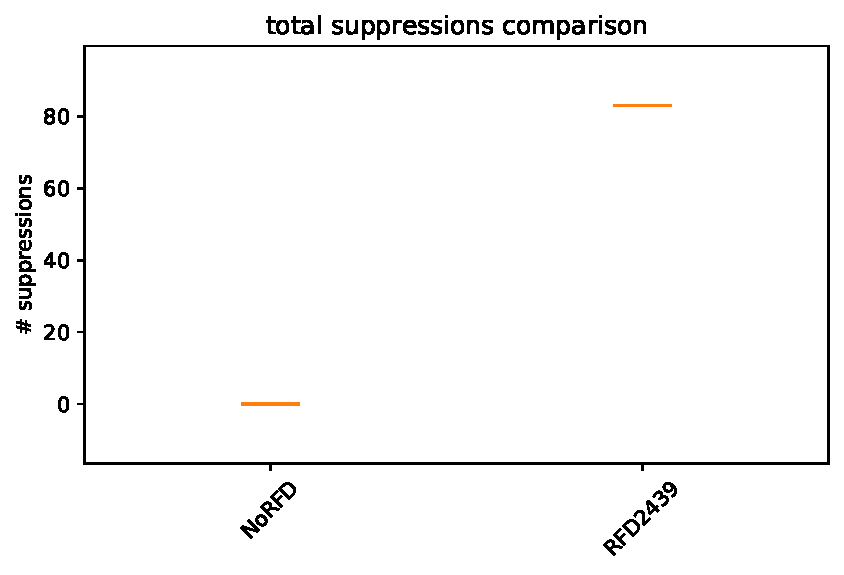
\includegraphics[width=\textwidth]{images/RFD/clique/clique_rfd_comparison_2439_suppressions_boxplot.pdf}
         \caption{Number of suppressions}
         \label{fig:RFD_2439_clique_MRAI30_suppressions}
     \end{subfigure}
        \caption{Clique topology, MRAI=30s, 10 runs, comparison of the network performances}
        \label{fig:RFD_2439_MRAI30}
\end{figure}

In \Cref{fig:RFD_2439_MRAI30} is possible to see a comparison between the use
of the standard \ac{RFD} and the completely deactivation of it.
The technique \textit{NoRFD} refers to experiments executed without the
\ac{RFD} mechanisms.
This comparison goal is to show the positive effects of this technique but also
the side effects of it.
In \Cref{fig:RFD_2439_clique_MRAI30_messages} is possible to see the advantages
of \ac{RFD} while the counter effects are presented in \Cref{fig:RFD_2439_clique_MRAI30_convTime}.
The number of messages transmitted with \ac{RFD} active are half of the \textit{NoRFD}
case, while, on the other hand, the averge convergence time of the entire network
is more than the double.
In \Cref{fig:RFD_2439_clique_MRAI30_suppressions} is possible to see the total
number of suppression executed on the entire network.
The \ac{RFD} mechanism keeps track of a different figure of merit for each neighbour,
because of that is possible that a node activate multiple suppression.
The total number of suppression activated by this environment is constant around
\num{82}.

In our case, the suppression on nodes \num{0} and \num{5} play an important role
for the network performances.
The first one for the spreading in the whole network, the second one for the
transmission of information to node $x$.

For this reason, the figure of merit evolution evolution of node \(x\) and five
is presented in \Cref{fig:clique_nodex_30,fig:clique_node5_30}, through it is
possible to analyze the different events effects.
The blue points represent that the route has not been suppressed yet.
Red points represent that the figure of merit has overpassed the suppression
thresholds and the route has been blocked.

\begin{figure}[h]
     \centering
     \begin{subfigure}[b]{0.476\textwidth}
         \centering
         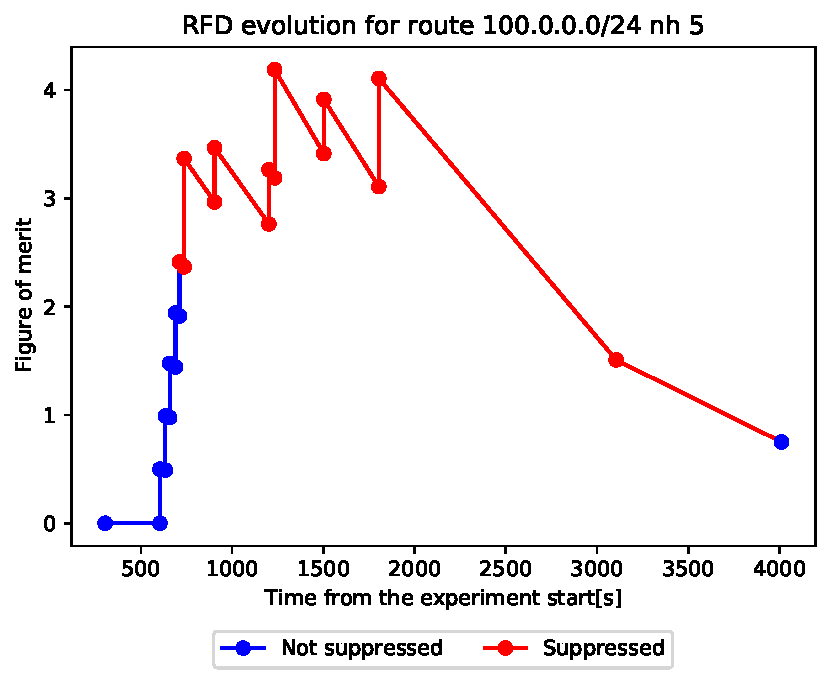
\includegraphics[width=\textwidth]{images/RFD/clique/FigureOfMerit/mrai7_RFD_x_rfd_R1.pdf}
         \caption{Node $x$ figure of merit evolution}
         \label{fig:clique_nodex_30}
     \end{subfigure}
     \hfill
     \begin{subfigure}[b]{0.494\textwidth}
         \centering
         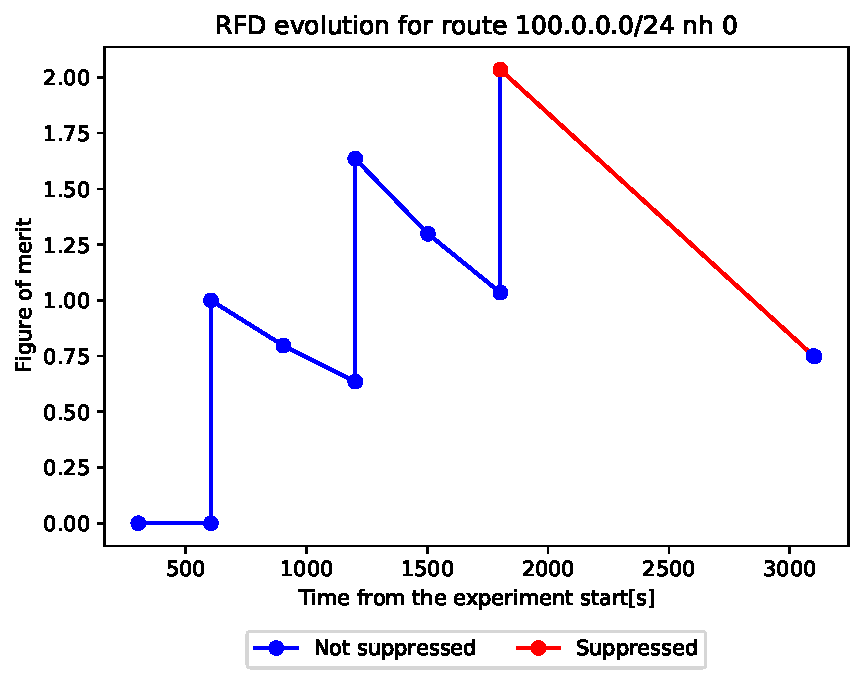
\includegraphics[width=\textwidth]{images/RFD/clique/FigureOfMerit/mrai7_RFD_5_rfd_R4.pdf}
         \caption{Node $5$ figure of merit evolution}
         \label{fig:clique_node5_30}
     \end{subfigure}
        \caption{Clique topology, MRAI=30s, figure of merit evolution
		of node \(x\) and node \num{5}}
        \label{fig:RFD_2439_figure_of_merit}
\end{figure}

In \Cref{fig:RFD_2439_figure_of_merit} is possible to see the two different
evolution, one of node \num{5} and the other from $x$.
Node \num{5} is the only servicer of $x$ for this reason every time it changes
its best path to reach the destination it sends an \ac{ADV} to $x$.
But, all this changes are interpreted as flaps by the \ac{RFD} filter of $x$,
because of that, the figure of merit grows very quickly.
It is sufficient a single case of \textit{Path Exploration} to provoke the
suppression of the route in $x$.
In \Cref{fig:clique_node5_30} is possible to see the evolution of the best path
of node \num{5}, the path that comes directly from \num{0}.
It takes more time for \num{5} to suppress this route, only the last flap
makes the figure of merit reach the suppression threshold.
In the same instant, around \SI{1800}{\second} also the route of $x$ gets the
last flap from \num{5} after that there is only one more point of variation
around \SI{3000}{\second}.
This last point correspond to the instant where the best route becomes available
again for \num{5}, at this point node $x$ receives the last \ac{ADV}.
But $x$ will need another \SI{1000}{\second} to makes the route available again.

Those two figure of merit evolutions show how one depends on the other.
The evolution of $x$ strictly depend on the one from \num{5}.
And also the network performances are highly affected by that, mostly the convergence
time, because further nodes from the source will take more time to converge making
the route available again.

\section{RFC 2439 VS RFC 7196}
\label{sec:rfd_2439_Vs_7196}

%\begin{itemize}
%		\item Present RFC 7196
%		\item Experiments clique with RFC 7196 MRAI=30
%		\item Node x and 5 figure of merit
%		\item RFC 2439 VS 7196
%\end{itemize}

The differences in the two \acp{RFC} that defines \ac{RFD} \cite{rfc2439,rfc7196}
are in the parameters used.
In fact, the \ac{RFC} \num{7196} modifies the figure
of merit threshold that is increased up to at least \num{6.0}, introducing
two new set of possible \ac{RFD} implementations that can be used:
\begin{itemize}
	\item \textit{\textbf{Aggressive}:} Suppression threshold no less than \num{6.0};
	\item \textit{\textbf{Conservative}:} Suppression threshold no less than \num{12.0}.
\end{itemize}
Respectively \num{3} and \num{6} times the actual standard.

I have then repeated the same experiments of \Cref{sec:rfd_toy_topologies} on the same
clique graph, but with the two new \ac{RFD} strategies.
The comparison between the different strategy performances is presented in \Cref{fig:RFD_MRAI30}.

\begin{figure}[h]
     \centering
     \begin{subfigure}[b]{0.49\textwidth}
         \centering
         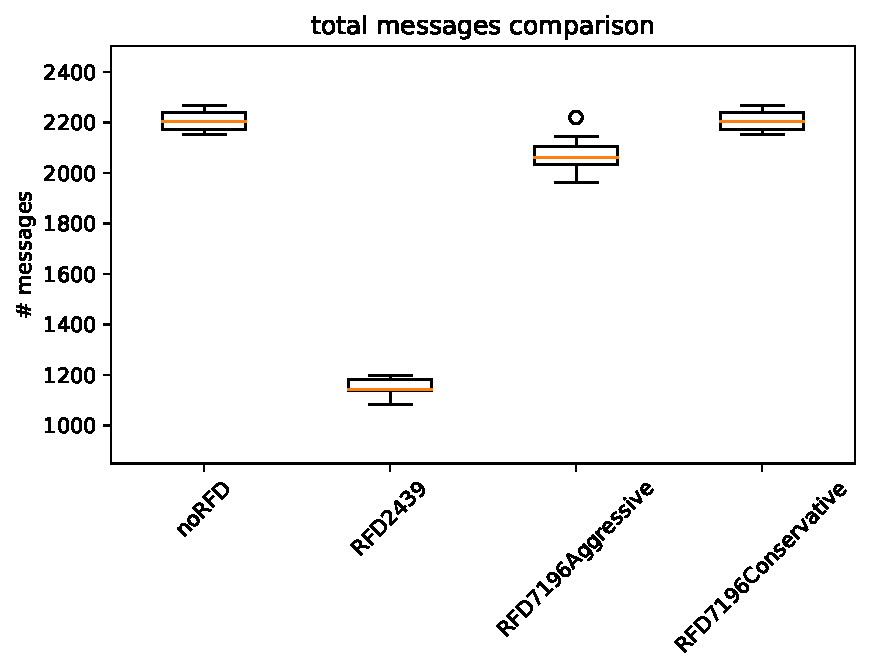
\includegraphics[width=\textwidth]{images/RFD/clique/clique_rfd_comparison_messages_boxplot.pdf}
         \caption{Messages comparison}
         \label{fig:RFD_clique_MRAI30_messages}
     \end{subfigure}
     \hfill
     \begin{subfigure}[b]{0.49\textwidth}
         \centering
         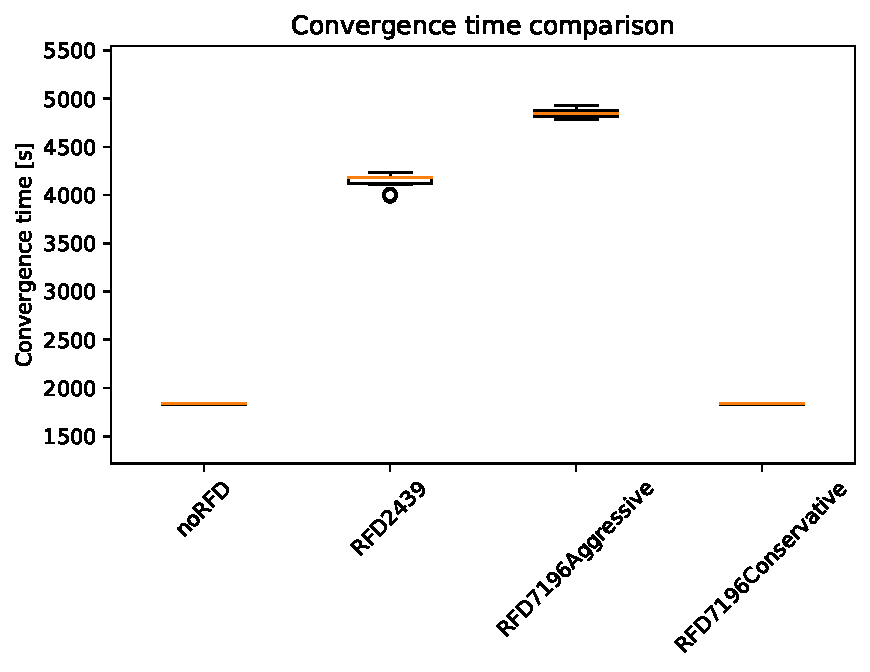
\includegraphics[width=\textwidth]{images/RFD/clique/clique_rfd_comparison_time_boxplot.pdf}
         \caption{Convergence time}
         \label{fig:RFD_clique_MRAI30_convTime}
     \end{subfigure}
     \hfill
     \begin{subfigure}[b]{0.49\textwidth}
         \centering
         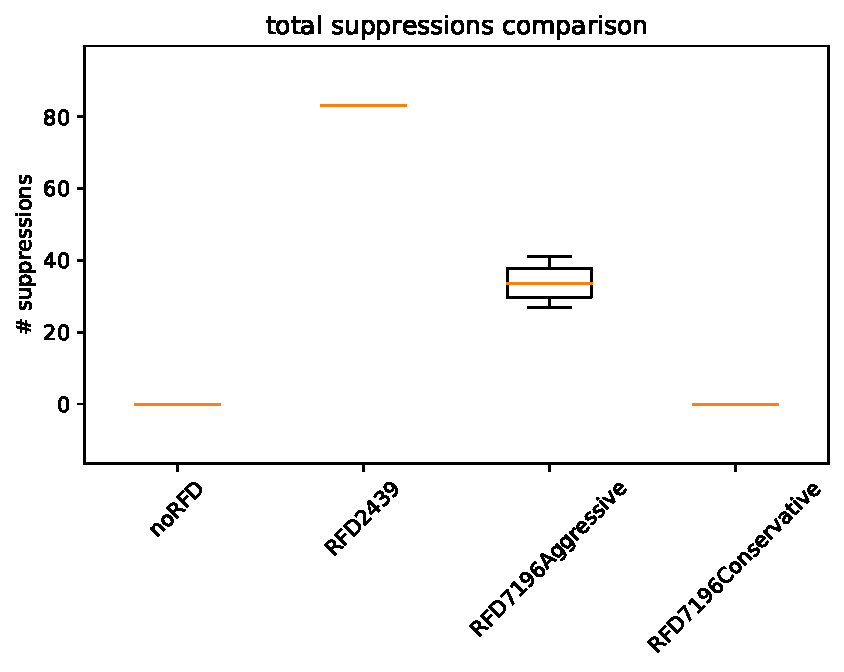
\includegraphics[width=\textwidth]{images/RFD/clique/clique_rfd_comparison_suppressions_boxplot.pdf}
         \caption{Number of suppressions}
         \label{fig:RFD_clique_MRAI30_suppressions}
     \end{subfigure}
		\caption{Clique topology, MRAI equal to \SI{30}{\second}, \num{10} runs,
				comparison of the network performances with all the \ac{RFD} strategies}
        \label{fig:RFD_MRAI30}
\end{figure}

In \Cref{fig:RFD_MRAI30} shows a complete comparison between all
the techniques.
Looking to \Cref{fig:RFD_clique_MRAI30_suppressions} is possible to notice that
the number of suppression can variate a lot changing the suppression threshold.
The \textit{Conservative} strategy doesn't trigger any suppression at all, while
the \textit{Aggressive} produces half the suppression of the legacy strategy.
Also, the \textit{Aggressive} strategy presents more variations in terms of
number of suppression.
Giving the fact that the conservative strategy doesn't trigger any suppression,
the results, in terms of performances, are equal to the case without \ac{RFD}.
The consequence in the number of suppression is noticeable also in
\Cref{fig:RFD_clique_MRAI30_messages}.
The \textit{Aggressive} strategy produce on average \num{2000} messages, almost
\num{1000} more of the configuration from the \ac{RFC} \num{2439}.

In \Cref{fig:RFD_clique_MRAI30_convTime} is possible to notice a strange behaviour.
I was expecting that having a lower number of suppression the \textit{Aggressive} strategy
would have obtained a convergence time lower than the standard \ac{RFD}, but,
this doesn't happened.
The cause is the fact that without modifying the decay function or the reuse
threshold, the figure of merit takes a longer time to become available again.

\section{Mice VS Elephants}
\label{sec:rfd_mice_vs_elephants}

%\begin{itemize}
%		\item Present mice and elephants
%		\item present experiments environment
%\end{itemize}

From the work of R. Bush et al., \cite{pelsser2011route} we know that the majority
of the \ac{ADV} that are transmitted on the Internet are from a small set of \acp{AS}.
Those \acp{AS} with their flaps cause update storms almost continuously.
I report a figure form \cite{pelsser2011route} for simplicity in
\Cref{fig:RBushPrefixes}.
Thanks to the studies of
\ac{APNIC}\footnote{\href{https://blog.apnic.net/2020/01/15/bgp-in-2019-bgp-churn/}{APNIC BGP 2019 report}}
is also known that this behaviour is still present nowadays, the \Cref{fig:apnicPrefixes}
is taken from one of their annual reports and shows that \num{10}\% of
all the active prefixes produce more or less the \num{70}\% of the total
messages detected.

\begin{figure}[h]
     \centering
     \begin{subfigure}[b]{0.48\textwidth}
         \centering
         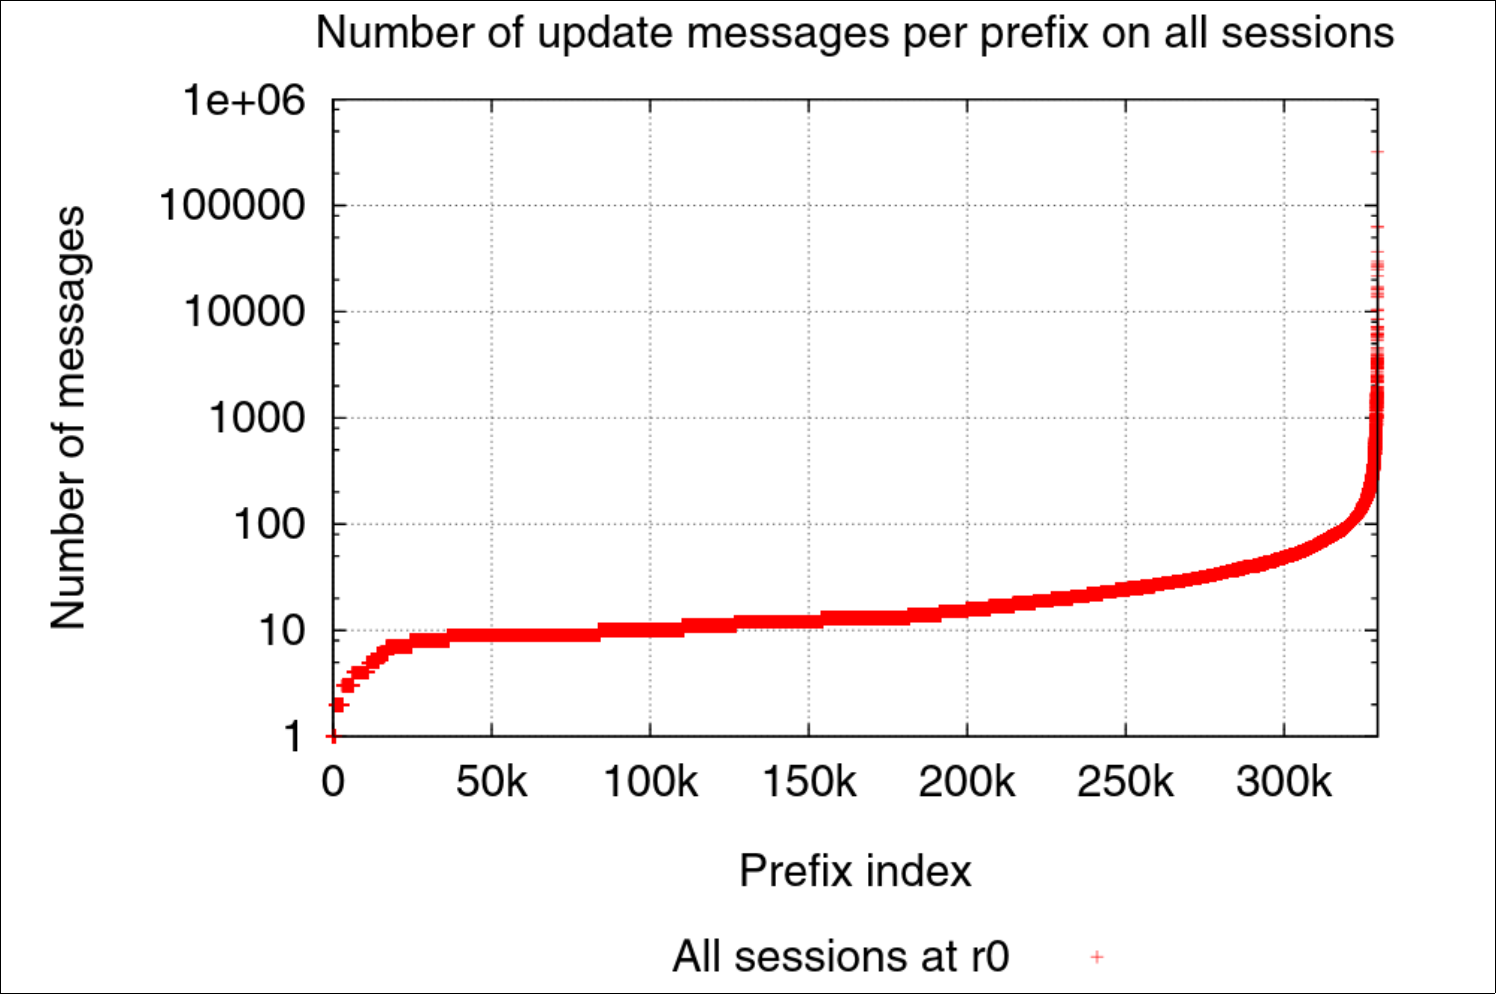
\includegraphics[width=\textwidth]{images/RFD/miceVSelephants/prefixVSmessagesRbush.png}
		 \caption{Prefixes and number of updates associated, figure from \cite{pelsser2011route}}
         \label{fig:RBushPrefixes}
     \end{subfigure}
     \hfill
     \begin{subfigure}[b]{0.50\textwidth}
         \centering
         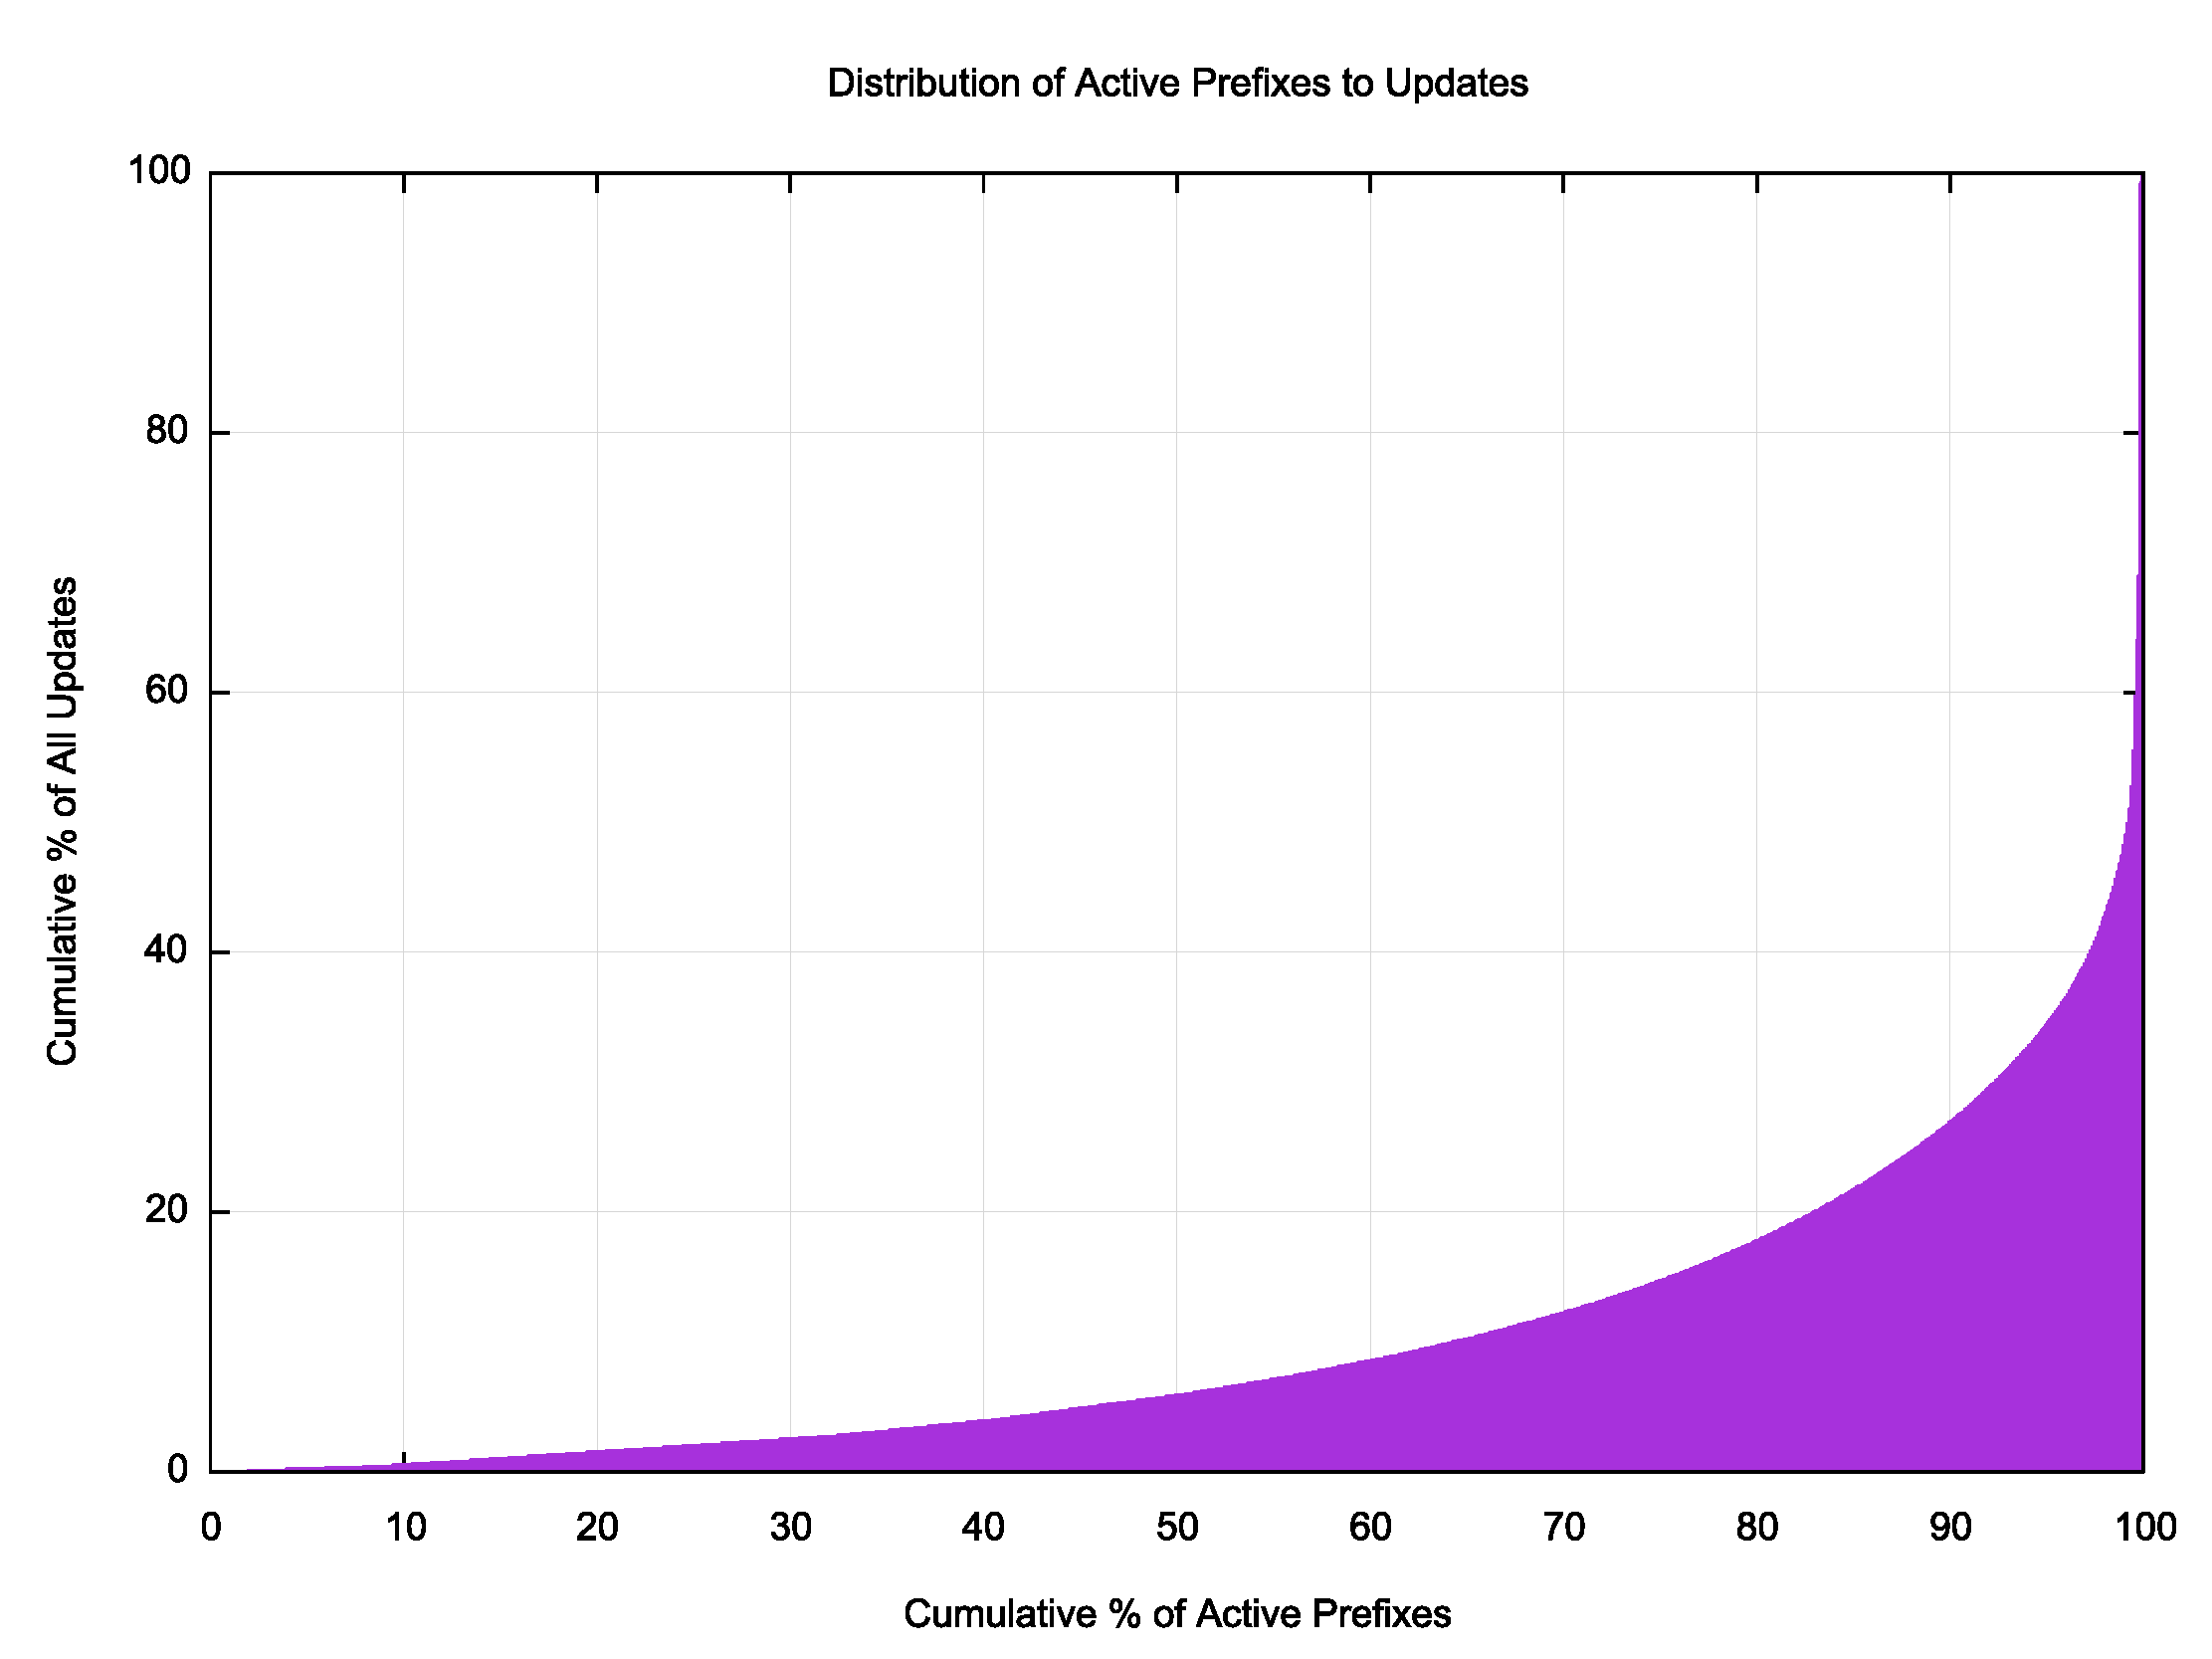
\includegraphics[width=\textwidth]{images/RFD/miceVSelephants/bgp2fig5-pfx-upds-cuml.png}
         \caption{Prefixes and number of updates associated, [apnic 2019]}
         \label{fig:apnicPrefixes}
     \end{subfigure}
        \caption{Prefixes influence on updates}
        \label{fig:prefixVSmessages}
\end{figure}

All the prefixes are then divisible in two sets:
\begin{itemize}
	\item \textbf{\textit{Mice}:} This set represent the majority of them,
		all the prefixes that does not generate more than \num{100} updates
		in \Cref{fig:RBushPrefixes};
	\item \textbf{\textit{Elephants}:} This set represent the remaining part
		of the prefixes, those that produces the majority of the messages.
\end{itemize}

Thanks to an annual review of \ac{BGP} by \ac{APNIC}, presented at \ac{RIPE}
\num{52}~\cite{huston2006bgp},
we can also have an example of those elephants prefixes.
This example is shown in \Cref{fig:ripePrefixFlaps}, it takes in consideration the
prefix \q{202.64.49.0/24} showing that in a relatively small period of time it has
produced thousands of \ac{ADV} per day.
In this case, this particular prefix has produced \num{198,370} \ac{ADV},
in total \num{96,330} flaps, in one year.

\begin{figure}[h]
    \centering
    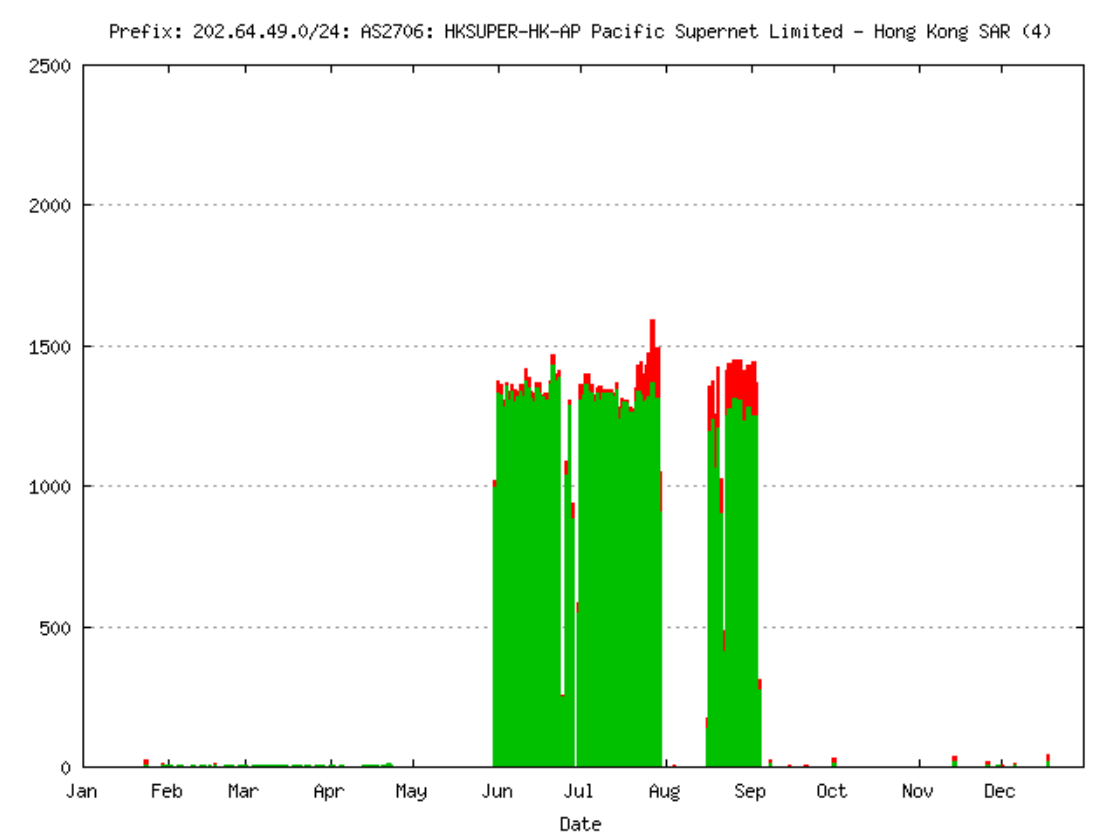
\includegraphics[scale=0.22]{images/RFD/miceVSelephants/ripePrefixFlap.png}
		\caption{202.64.49.0/24 flaps plot from \ac{RIPE} 52~\cite{huston2006bgp}}
    \label{fig:ripePrefixFlaps}
\end{figure}

I have then used this data to configure two new environments for the simulations.
The first one points to reproduce the \textit{Mice} behaviour, the second
one the \textit{Elephants}.

In both these environments, I have then compared the four different strategies
saw in \Cref{sec:rfd_toy_topologies,sec:rfd_2439_Vs_7196}: \textit{NoRFD},
standard \ac{RFD} from the \ac{RFC} \num{2439} and the two updated versions
from the \ac{RFC} \num{7196}~\cite{rfc7196}.

The topology used for those experiments is an \textit{Internet like} topology
with \num{1000} nodes and \ac{MRAI} is fixed to \SI{30}{\second} for all the links.
The source of the signal has been chosen randomly on the graph.
For each experiment has been executed \num{50} runs.


\subsection{Mice}
\label{subsec:rfd_mice}

%\begin{itemize}
%		\item Present mice environment
%		\item mice experiments with MRAI=30
%\end{itemize}
The particularity of the \textit{Mice} experiments is in the signal, it contains
few flaps interleaved by a large time interval.
I have then used a signal with \num{5} flaps, \q{AWAWAWAWAWA} with a delay
of \SI{300}{\second} (\SI{5}{\minute}) between each message.
The results are presented in \Cref{fig:1000_RFD_MRAI30_mice_bis}.
I have executed \num{50} runs for each \ac{RFD} strategy.

\begin{figure}[h]
     \centering
     \begin{subfigure}[b]{0.49\textwidth}
         \centering
         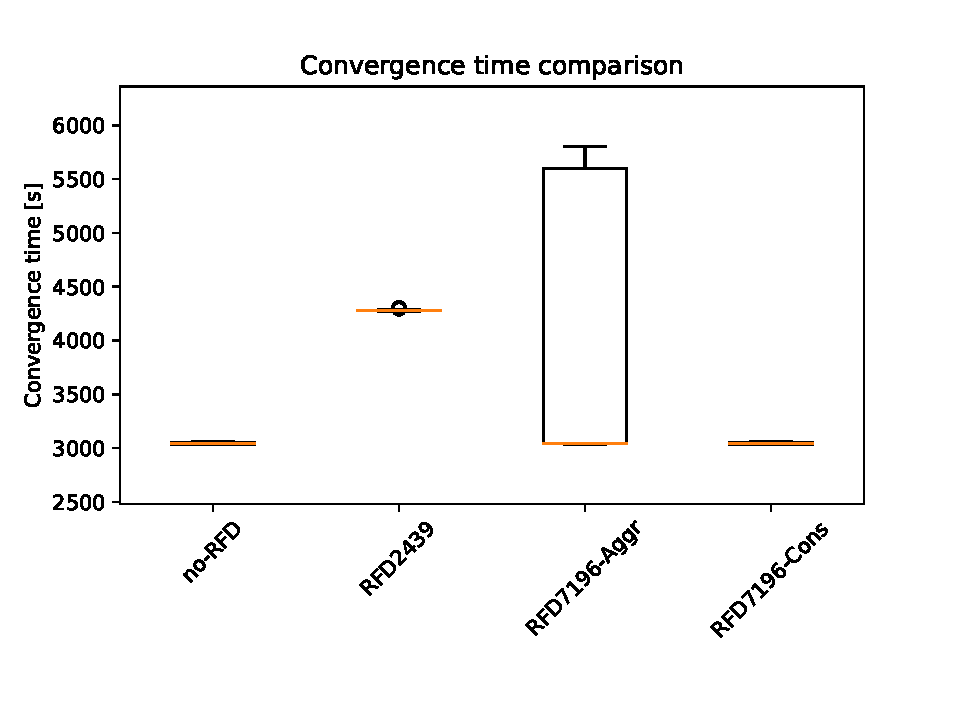
\includegraphics[width=\textwidth]{images/RFD/miceVSelephants/mice/cisco_1000MRAI30_rfd_comparison_time_boxplot.pdf}
         \caption{Convergence time respect to the RFD strategy}
         \label{fig:1000_RFD_MRAI30_mice_time_bis}
     \end{subfigure}
     \hfill
     \begin{subfigure}[b]{0.49\textwidth}
         \centering
         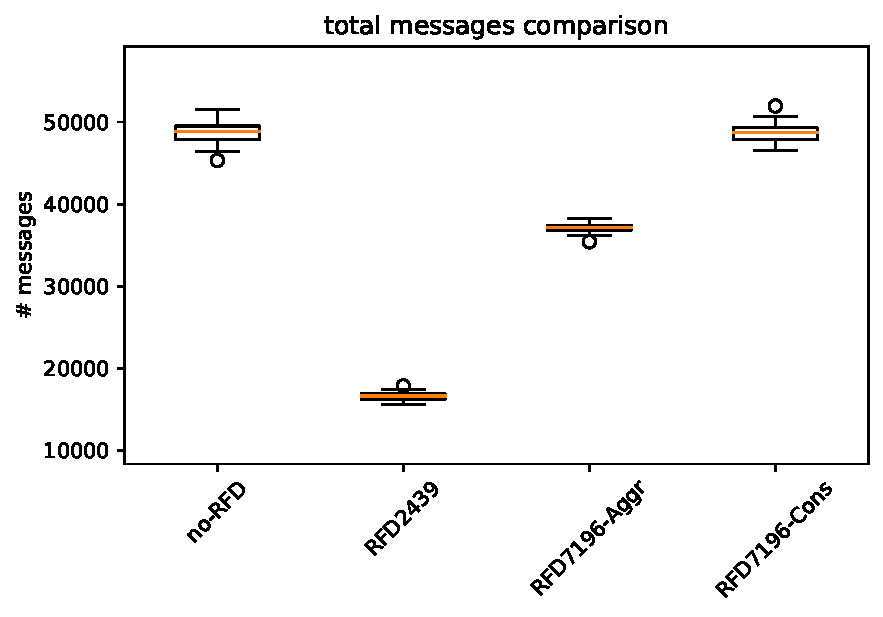
\includegraphics[width=\textwidth]{images/RFD/miceVSelephants/mice/cisco_1000MRAI30_rfd_comparison_messages_boxplot.pdf}
         \caption{Number of messages respect to the RFD strategy}
         \label{fig:1000_RFD_MRAI30_mice_messages_bis}
     \end{subfigure}
     \begin{subfigure}[b]{0.49\textwidth}
         \centering
         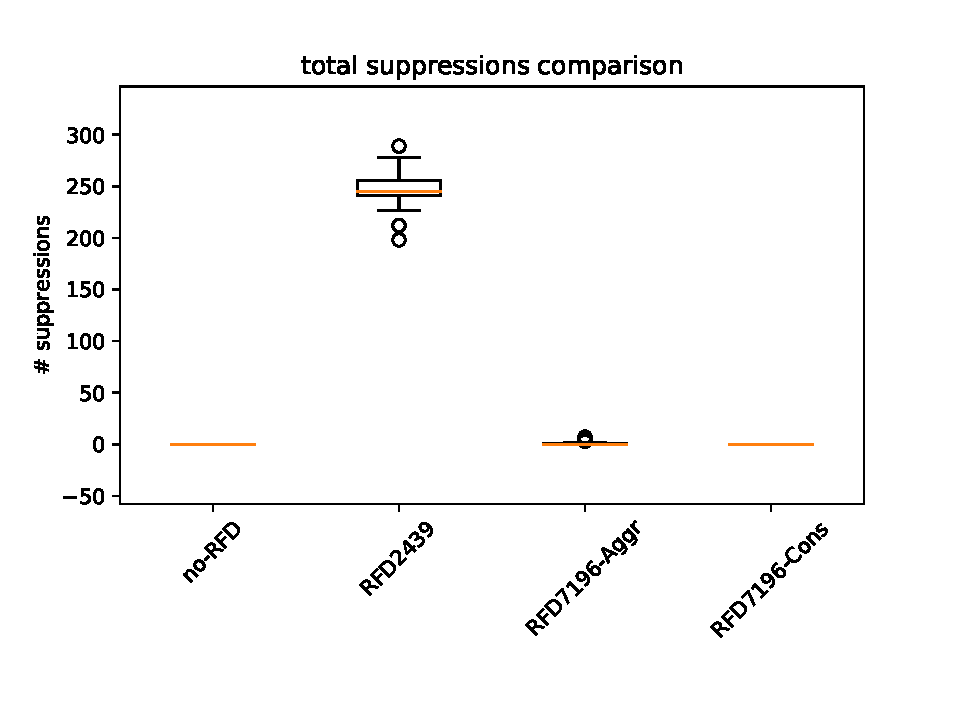
\includegraphics[width=\textwidth]{images/RFD/miceVSelephants/mice/cisco_1000MRAI30_rfd_comparison_suppressions_boxplot.pdf}
         \caption{Number of suppressions respect to the RFD strategy}
         \label{fig:1000_RFD_MRAI30_mice_suppressions_bis}
     \end{subfigure}
		\caption{Internet like topology 1000 nodes, MRAI=30s, random destination,
		5 flaps \q{AWAWAWAWAWA}, \SI{300}{\second} message delay, Network performances,
		\num{50} runs per strategy.}
        \label{fig:1000_RFD_MRAI30_mice_bis}
\end{figure}

From \Cref{fig:1000_RFD_MRAI30_mice_suppressions_bis} is possible to see that
there is a big difference in the number of suppression.
The standard strategy produces on average almost \num{1500} suppressions and the effects
of those suppressions can be seen in \Cref{fig:1000_RFD_MRAI30_mice_time_bis,fig:1000_RFD_MRAI30_mice_messages_bis}.
On average, it presents a convergence time higher than \SI{6000}{\second}
but with a number of total messages transmitted around \num{16000} with a very
low variance.
A different case is presented by the \textit{Conservative} strategy from \ac{RFC}
7196 \cite{rfc7196}.
The threshold in this last case is so permissive that produces a really small
number of suppression.
For this reason, the number of messages transmitted, on average, is similar to
the \textit{NoRFD} case, around \num{50000}.
While, the convergence time is around \SI{6500}{\second}, like the standard \ac{RFD}
strategy.
This proves that few suppression can heavily influence the network performances,
in particular the convergence time.
Also because the recover from a suppression with a higher threshold would require
more time.

In the middle there is the \textit{Aggressive} strategy, from the
suppression boxplot is noticeable that it produces a smaller number of suppression in respect
of the legacy strategy with a smaller variance.
Also, the convergence time respect this trend, in fact, the average time is
below \SI{6000}{\second}.
While The number of messages transmitted is more than double in respect
of the strategy described by the \ac{RFC} \num{2439}.

In conclusion, I can say that a small number of suppression can affect the
performances, like the few suppressions in the \textit{Conservative} strategy
for the convergence time.
Also, the few missing suppression in the \textit{Aggressive} strategy will
enormously impact the number of messages transmitted.

Is also possible to study which are the nodes that produce the suppression and how
far are them from the signal source.
The results of this study, for each suppression technique, are presented
in \Cref{fig:1000_RFD_centVSsup}.

\begin{figure}[h]
     \centering
     \begin{subfigure}[b]{0.49\textwidth}
         \centering
         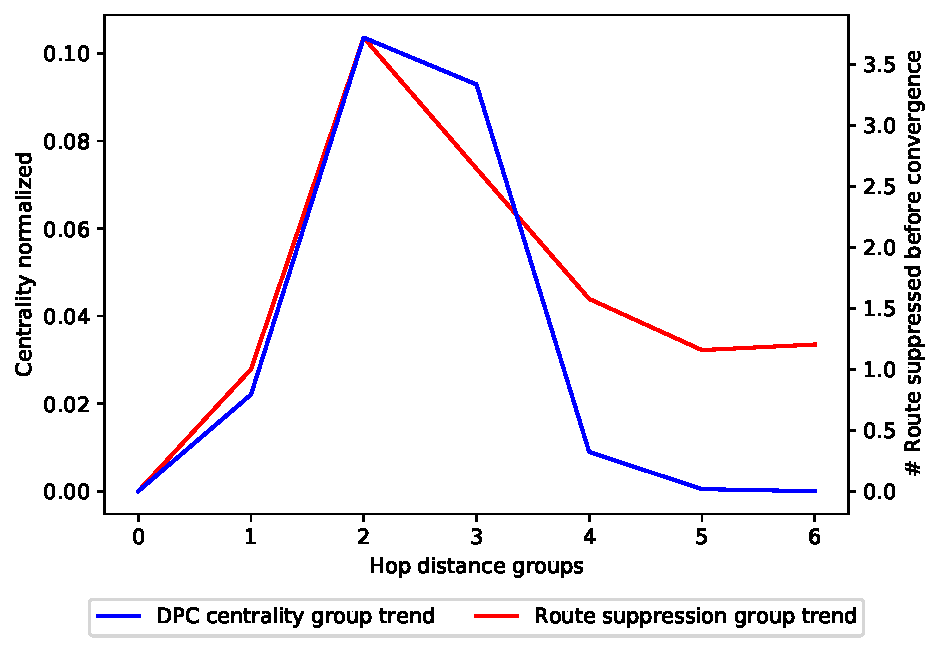
\includegraphics[width=\textwidth]{images/RFD/miceVSelephants/mice/cisco_1000_RFD_nodeConvergence_centVSsup_trend.pdf}
         \caption{RFD 2439 Strategy}
         \label{fig:1000_2439RFD_centVSsup}
     \end{subfigure}
     \hfill
     \begin{subfigure}[b]{0.49\textwidth}
         \centering
         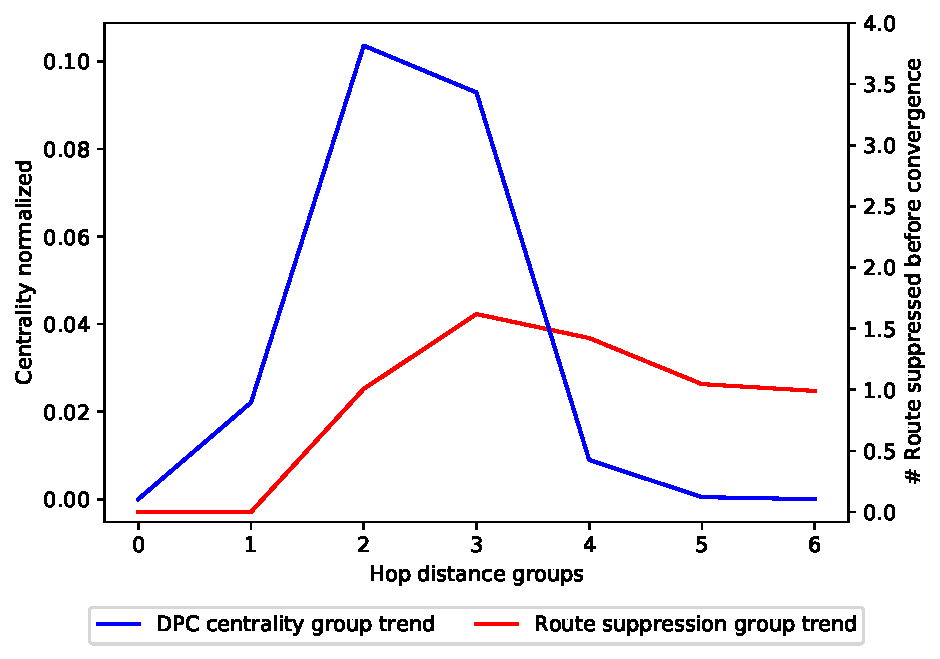
\includegraphics[width=\textwidth]{images/RFD/miceVSelephants/mice/cisco_1000_RFD_7196_aggressive_nodeConvergence_centVSsup_trend.pdf}
         \caption{RFD 7196 Aggressive Strategy}
         \label{fig:1000_7196RFDA_centVSsup}
     \end{subfigure}
     \hfill
     \begin{subfigure}[b]{0.49\textwidth}
         \centering
         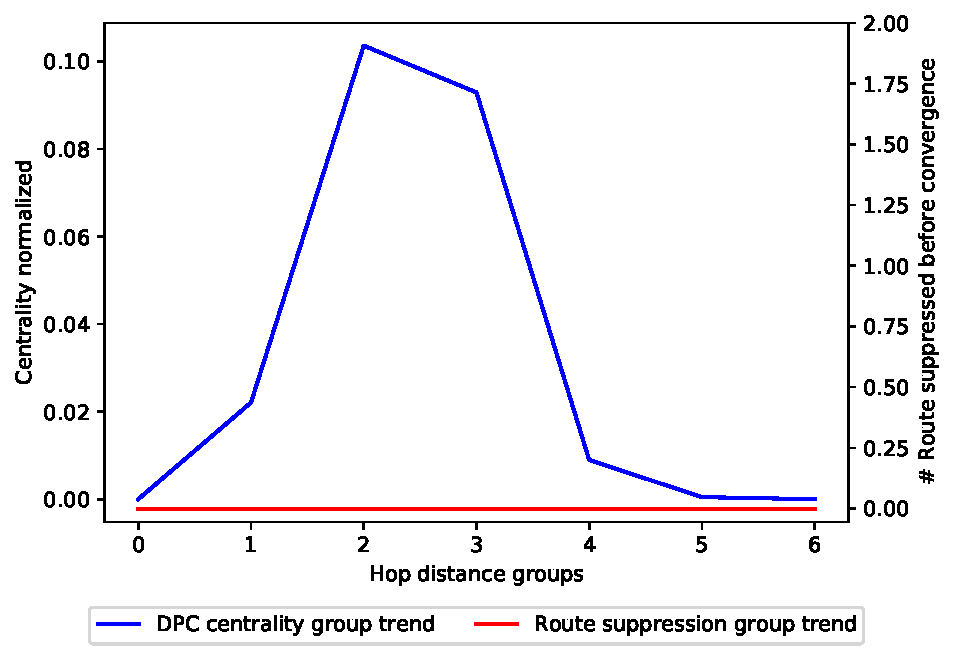
\includegraphics[width=\textwidth]{images/RFD/miceVSelephants/mice/cisco_1000_RFD_7196_conservative_nodeConvergence_centVSsup_trend.pdf}
         \caption{RFD 7196 Conservative Strategy}
         \label{fig:1000_7196RFDC_centVSsup}
     \end{subfigure}
		\caption{Internet like topology \num{1000} nodes, \ac{MRAI} = \SI{30}{\second},
		random destination, \num{5} flaps, \SI{300}{\second} between messages,
		Suppression trend VS avg hop distance from the source}
        \label{fig:1000_RFD_centVSsup}
\end{figure}

For the plots in \Cref{fig:1000_RFD_centVSsup} the $x$ axis represent the distance
from the source node in terms of hops, all the nodes are grouped by this
distance.
The blue line represents the average centrality of the groups, for each node of the
graph I calculated the centrality using the \ac{DPC} metric and then grouped them
by the distance and calculated the average value.
As expected the central nodes have a higher centrality and are a few hops
of distance from the source node.
The centrality trend is equal for each plot in \Cref{fig:1000_RFD_centVSsup}
because the graph and the source node are the same for each experiment.

The red line represents the average number of suppression per group.
With the standard strategy, \Cref{fig:1000_2439RFD_centVSsup},
on average, the route has been blocked \num{1} time by the nearest nodes and then,
this value increase reaching the center clique up to \num{3.5} times and then
slowly decreases in the following groups.
In the farthest group, on average, is possible to notice \num{1} suppression.

The \textit{Aggressive} strategy, \Cref{fig:1000_7196RFDA_centVSsup}, present
a similar behaviour, the nearest nodes don't block the route, while the central
nodes start blocking it, on average at least \num{1} time.
After those central nodes, the farthest nodes, that have a low centrality, will
block it on average \num{1} time, like the legacy strategy.

The \textit{Conservative} strategy, presented in \Cref{fig:1000_7196RFDC_centVSsup},
has a different trend.
The central nodes do not block the route, while only the farthest
ones block it a few times, with an average value of \num{0.2} times.
This can give us some hints, a very high threshold can promote the path
exploration problem that will cause multiple update storms in farthest nodes.
The suppression on the furthest nodes are the cause to the high convergence time,
because, all the other groups don't experience suppression and for this reason
they converge faster.

From those experiments, I can conclude that having a higher threshold could help
to spread the knowledge near the source of the flaps, but once the
\textit{Path exploration} problem takes over, the nodes are going to suppress
the destination.
Those few suppression can highly impact in general the entire network enlarging
the average convergence rate of the nodes.
Is important to consider that a higher threshold means also a higher time to
make the destination available again, maybe a new decay function should be considered.


\subsection{Elephants}
\label{subsec:rfd_elephants}

%\begin{itemize}
%		\item Present elephants environment
%		\item elephants experiments with MRAI=30
%\end{itemize}

The elephants prefixes, as I mentioned in \Cref{sec:rfd_mice_vs_elephants},
are the ones that produce the majority of the \ac{ADV}.
And, thanks to \cite{huston2006bgp}, is also known that is possible to see over
thousands of messages per day.
For this reason, the \textit{elephants} environment signal is composed of \num{100}
flaps, with a delay between the messages of \SI{3}{\second}.
All the other properties of the environment are unchanged.
The results are presented in \Cref{fig:1000_RFD_MRAI_30_elephant,fig:1000_RFD_cent_VS_sup_elephants}.

\begin{figure}[h]
     \centering
     \begin{subfigure}[b]{0.49\textwidth}
         \centering
         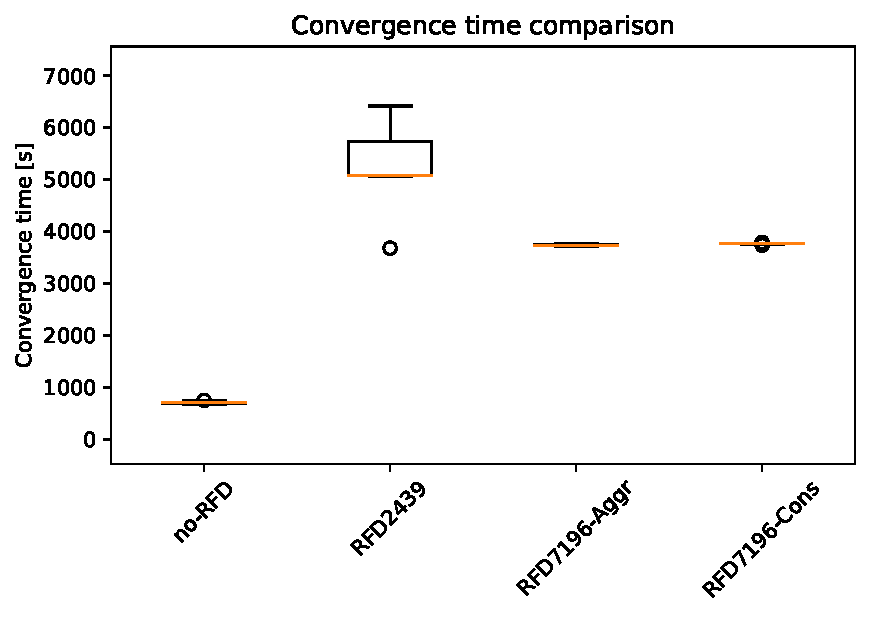
\includegraphics[width=\textwidth]{images/RFD/miceVSelephants/elephants/cisco_1000MRAI30_rfd_comparison_time_boxplot.pdf}
         \caption{Convergence time respect to the RFD strategy}
         \label{fig:1000_RFD_MRAI_30_time_elephant}
     \end{subfigure}
     \hfill
     \begin{subfigure}[b]{0.49\textwidth}
         \centering
         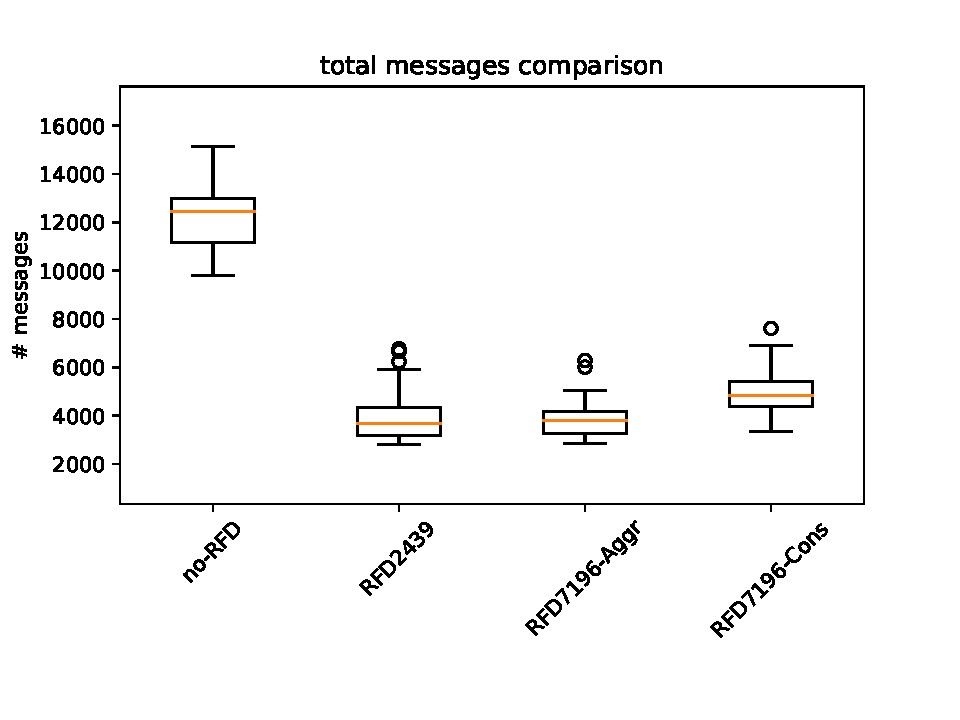
\includegraphics[width=\textwidth]{images/RFD/miceVSelephants/elephants/cisco_1000MRAI30_rfd_comparison_messages_boxplot.pdf}
         \caption{Number of messages respect to the RFD strategy}
         \label{fig:1000_RFD_MRAI_30_messages_elephant}
     \end{subfigure}
     \begin{subfigure}[b]{0.49\textwidth}
         \centering
         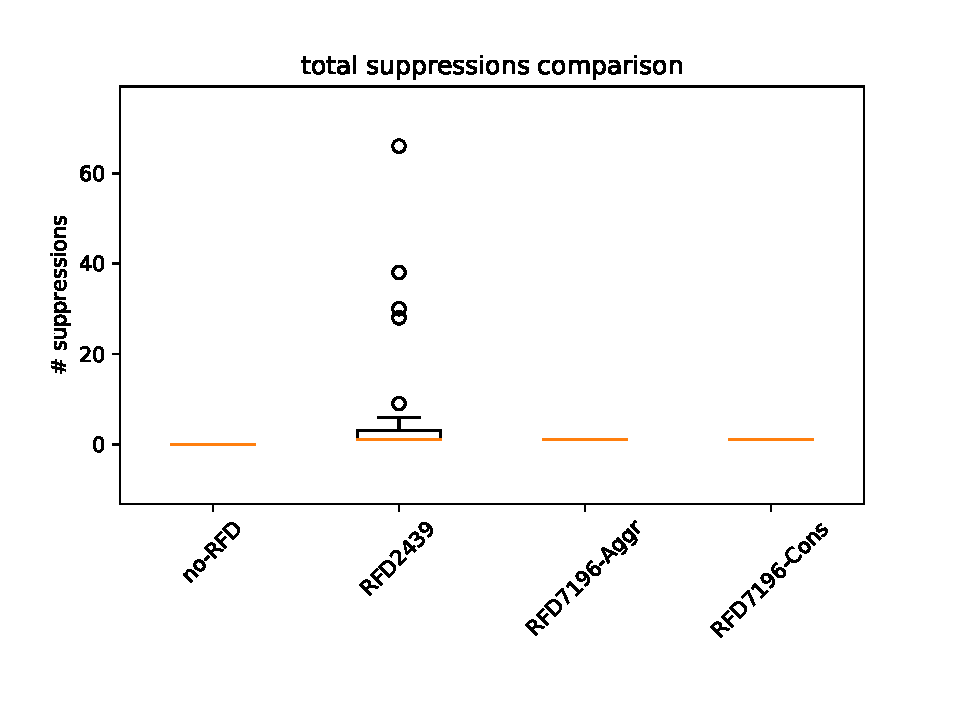
\includegraphics[width=\textwidth]{images/RFD/miceVSelephants/elephants/cisco_1000MRAI30_rfd_comparison_suppressions_boxplot.pdf}
         \caption{Number of suppressions respect to the RFD strategy}
         \label{fig:1000_RFD_MRAI_30_suppressions_elephant}
     \end{subfigure}
		\caption{Network performances, Internet like topology \num{1000} nodes, \ac{MRAI} = \SI{30}{\second},
		random destination, \num{100} flaps, \SI{3}{\second} delay between each
		message, \num{50} runs for each strategy}
        \label{fig:1000_RFD_MRAI_30_elephant}
\end{figure}

In \Cref{fig:1000_RFD_MRAI_30_elephant} is possible to see that this time
all the \num{3} \ac{RFD} strategies produce a different behaviour.
In \Cref{fig:1000_RFD_MRAI_30_suppressions_elephant}
the standard strategy, on average, triggers more than \num{1250} suppression, producing
the lowest number of messages, around \num{11000}, but the highest convergence
time with more than \SI{5000}{\second}.
All the suppression are triggered by the \textit{Path Exploration} problem that
causes \ac{ADV} storms that provoke, on the majority of the nodes, an overpass
of the critical threshold.
The two new strategies would produce on average just few suppression in respect
of the legacy one, but the number of messages doesn't differ too much.
While there is a huge improvement on the convergence time, on average,
both the new strategy permits the network to converge in less than \SI{4000}{\second}.
All three strategies produce $1/3$ of the messages transmitted by the completely
absence of the \ac{RFD}.

\begin{figure}[h]
     \centering
     \begin{subfigure}[b]{0.49\textwidth}
         \centering
         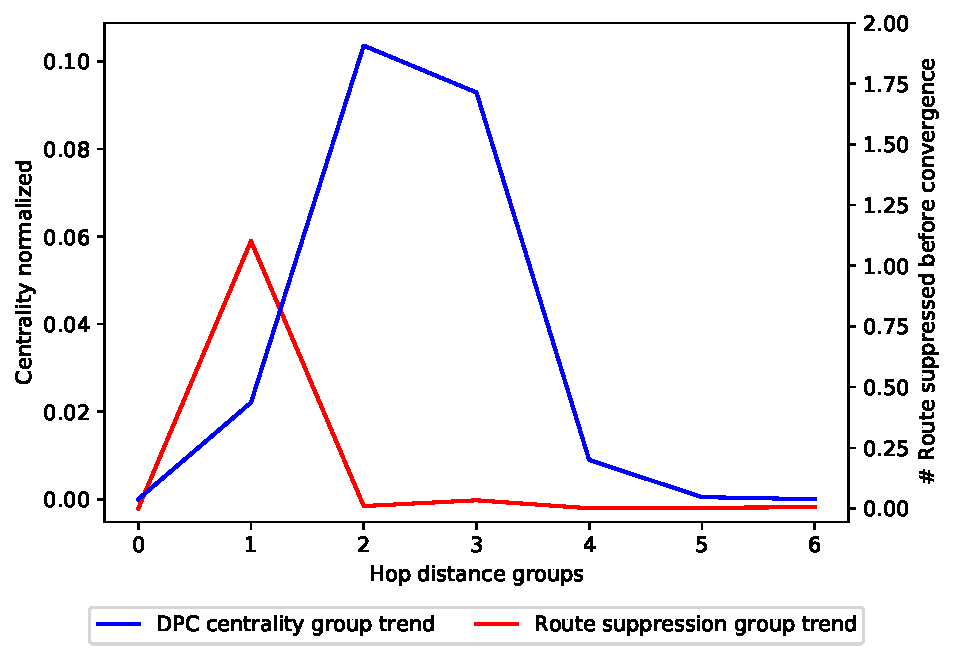
\includegraphics[width=\textwidth]{images/RFD/miceVSelephants/elephants/cisco_1000_RFD_nodeConvergence_centVSsup_trend.pdf}
         \caption{RFD 2439 Strategy}
         \label{fig:1000_2439RFD_cent_VS_sup_elephants}
     \end{subfigure}
     \hfill
     \begin{subfigure}[b]{0.49\textwidth}
         \centering
         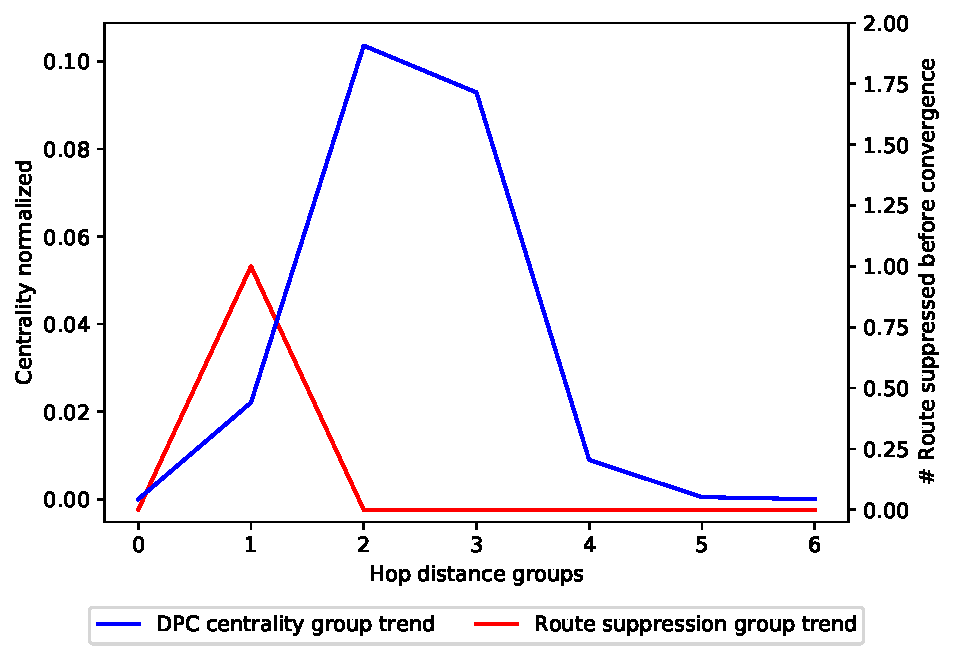
\includegraphics[width=\textwidth]{images/RFD/miceVSelephants/elephants/cisco_1000_RFD_7196_aggressive_nodeConvergence_centVSsup_trend.pdf}
         \caption{RFD 7196 Aggressive Strategy}
         \label{fig:1000_7196RFDA_cent_VS_sup_elephants}
     \end{subfigure}
     \hfill
     \begin{subfigure}[b]{0.49\textwidth}
         \centering
         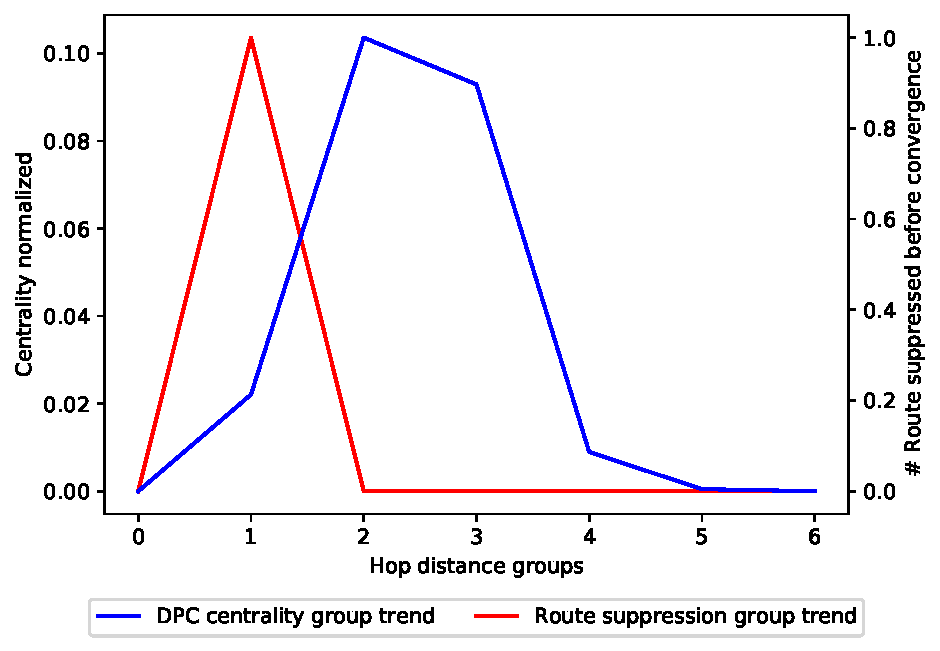
\includegraphics[width=\textwidth]{images/RFD/miceVSelephants/elephants/cisco_1000_RFD_7196_conservative_nodeConvergence_centVSsup_trend.pdf}
         \caption{RFD 7196 Conservative Strategy}
         \label{fig:1000_7196RFDC_cent_VS_sup_elephants}
     \end{subfigure}
		\caption{Internet like topology \num{1000} nodes, \ac{MRAI} = \SI{30}{\second},
		random destination, \num{100} flaps, \SI{3}{\second} delay between each
		message, suppressions by distance from the source in terms of hops.
		Each point is the average of all the values produced by the nodes at the
		same distance from the source.}
        \label{fig:1000_RFD_cent_VS_sup_elephants}
\end{figure}

In \Cref{fig:1000_RFD_cent_VS_sup_elephants} is presented the comparison between
the average number of suppression per node group of the different strategies.
In \Cref{fig:1000_7196RFDA_cent_VS_sup_elephants,fig:1000_7196RFDC_cent_VS_sup_elephants}
is possible to notice that both strategies, \textit{Aggressive} and \textit{Conservative},
reacts in the exact same way at the elephant environment.
The only nodes that suppress the route are the nodes that are closer to the source.
All the other nodes of the network don't experience enough messages to block
the route.

The first figure, \Cref{fig:1000_2439RFD_cent_VS_sup_elephants} shows
that, on average, every node suppress at least one time the source of the
signal.
The hypothesis behind this trend is that the number of messages that pass the
nearest nodes are enough to provoke a \textit{Path Exploration} behaviour and
with a small threshold those messages storms are enough to overcome the suppression
threshold.
With a lower threshold is sufficient a small number of \ac{ADV} storms
to trigger the \ac{RFD} suppression.

%We can then say that all the strategies catch in time the flap and avoid the
%propagation of the update storm, increasing the convergence time but protecting
%the network from thousands of messages.
With those experiments has been proven that all the strategies protect the
network from a huge load of messages.
\Cref{fig:1000_RFD_MRAI_30_messages_elephant} shows that the use of \ac{RFD}
reduces to $1/3$ the number of messages necessary to reach convergence.
The difference is in the convergence time, more nodes experience suppression
then more time is necessary to converge.
Because, there will be more \ac{ADV}, when
the figure of merit becomes lower enough to activate again the route the nodes
will provoke a new message storm.
For this reason there is a difference of more than \SI{1000}{\second} between
the techniques.
This experiments reinforce the hypothesis that a small number of suppressions is
more significant in respect of thousands of them.

